\subsection{Na\"{i}ve Approach}
We consider model parallelizing the DNN on a distributed-memory system using 
MPI. Figure~\ref{fig:altsplit_baseline} illustrates a na\"{i}ve approach to it 
which also serves as the baseline of our research. It depicts a 5-layer 
all-connected DNN split on two MPI processes and the 4 neurons per layer are 
evenly assigned to each MPI process. The input and output layer are omitted and 
we assume they are replicated in every MPI process. The black arrows in the 
figure indicate all-to-all communications between the two MPI processes. During 
both the forward- and backward-propagation, each neuron from the current layer 
needs the outputs of the entire neurons from the preceding layer. All-to-all 
communication will have to happen across all the MPI processes. In the figure, 
prior to the computation of each layer 4 all-to-all communication need to occur 
so that the output information from the preceding layer can get to be fully 
propagated to the respective portions of the current layer to all the MPI 
processes.  Albeit some numerical rounding error introduced by the all-to-all 
communication, this approach guarantees that the output information from the 
preceding layer is consistent and identical across all the MPI processes prior 
to the computation of their respective portions of the current layer.
\begin{figure}[H]
    \centerline{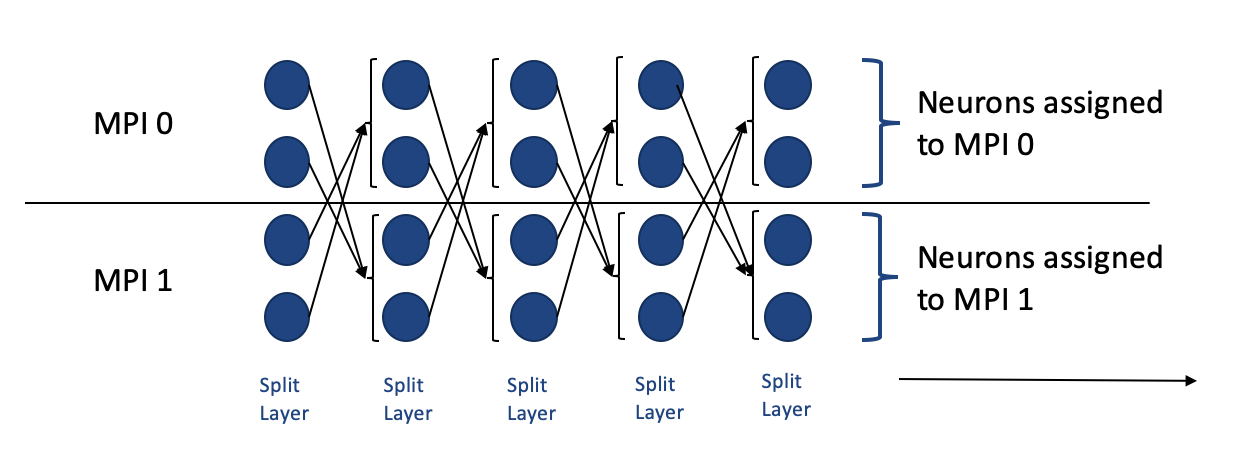
\includegraphics[scale=0.60]{altsplit/figs/baseline.png}}
    \caption{Baseline model parallelism scheme}
    \label{fig:altsplit_baseline}
\end{figure}

Algorithm~\ref{alg:altsplit_sequential}
\begin{algorithm}[H]%algorithm* occupies full page
\caption{Sequential DNN}
\label{alg:altsplit_sequential}
{\fontsize{10}{10}\selectfont
\begin{algorithmic}[1]
    \ForAll {$l \in layers[0:max]$}
    \Comment Foward phase
        \ForAll {$n \in neurons[0:max]$}
            \State Compute output
        \EndFor
    \EndFor
    \ForAll {$l \in layers[max:0]$}
    \Comment Backpropagation phase
        \ForAll {$n \in neurons[0:max]$}
            \State Compute gradient $\Delta W$
        \EndFor
    \EndFor
    \State Update parameters
\end{algorithmic}}
\end{algorithm}

\begin{algorithm}[H]
\caption{Na\"{i}ve model parallelism of DNN}
\label{alg:altsplit_baseline}
{\fontsize{10}{10}\selectfont
\begin{algorithmic}[1]
    \ForAll {$p \in MPI\_Processes$}
        \ForAll {$l \in layers[0:max]$}
        \Comment Foward phase
            \State MPI\_Allgather
            \ForAll {$n \in neurons_{p}$}
                \State Compute output
            \EndFor
        \EndFor
    \EndFor
    \ForAll {$p \in MPI\_Processes$}
        \ForAll {$l \in layers[max:0]$}
        \Comment Backpropagation phase
            \State MPI\_Allreduce
            \ForAll {$n \in neurons_{p}$}
                \State Compute gradient $\Delta W$
            \EndFor
        \EndFor
    \EndFor
    \ForAll {$p \in MPI\_Processes$}
        \State Update parameters
    \EndFor
\end{algorithmic}}
\end{algorithm}

\subsection{Altsplit (Alternate Split) Approach}
We propose the \emph{Altsplit} approach which splits or replicates the layers 
alternately. The scheme is illustrated in Figure~\ref{fig:altsplit_scheme} with 
the same 5-layer DNN as in Figure~\ref{fig:altsplit_baseline}. The first layer 
is split across MPI processes whereas the next layer is replicated over 
the MPI processes with the same initialization values. Subsequent layers are 
constructed with alternating splits and replications.

As in the na\"{i}ve approach, all-to-all communication has to happen if the 
preceding layer is split over the MPI processes. In order to 

\begin{figure}[H]
    \centerline{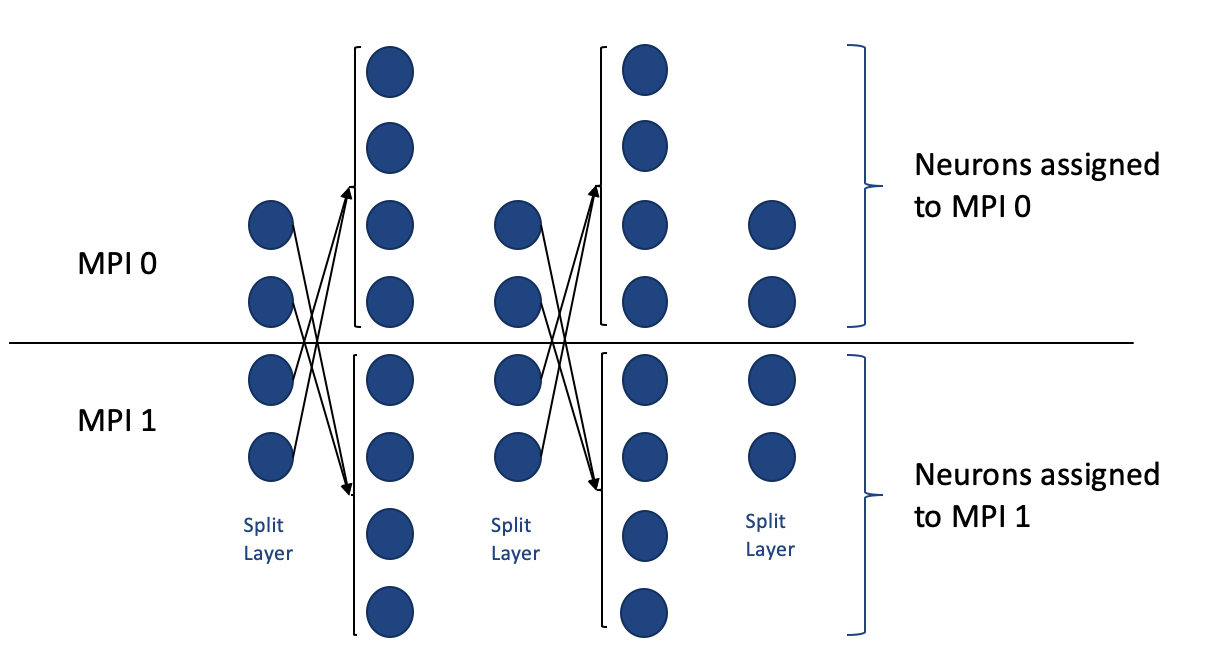
\includegraphics[scale=0.60]{altsplit/figs/altsplit.png}}
    \caption{The \emph{Altsplit} scheme}
    \label{fig:altsplit_scheme}
\end{figure}
